\chapter{Gravity Inversion}\label{Chp:cook:gravity inversion}

This part illustrates the use of gravity and magnetic inversion. This code was written in 2012 at the school of Earth science at University of Queensland.

It enables geologists and geophysicists, who are not necessarily well versed in the details of inversion theory, to process, visualize and interpret multi-volume geophysical data and modern visualization techniques. As well as being functional interpretation system, it is a research and development environment for geophysical analysis.

We present a package for inverting gravity and magnetic data from ground or airborne surveys to generate a 2-D or 3-D distribution of density and/or susceptibility contrast. With these codes, the earth is modeled using a large number of rectangular cells with constant values of density and susceptibility. The final distribution is obtained by minimizing a model objective function to fit the observed data.

This package could be used to provide models which introduce density and susceptibility together to fit a given set of magnetic and gravity anomalies. The given data might contain negative and positive values for both onshore and offshore regions. The model is a 3-dimensional and any cross or depth sections are extracted from. One of the advantages of this package is the ability to process both big and small areas.

All corrections and processing should be completed befor the data is fed to our system. Model is described as big volume which has varying in density and susceptibility smoothly in all directions. The apparent characteristics of the topography are very sophisticated.


\begin{figure}
\centering
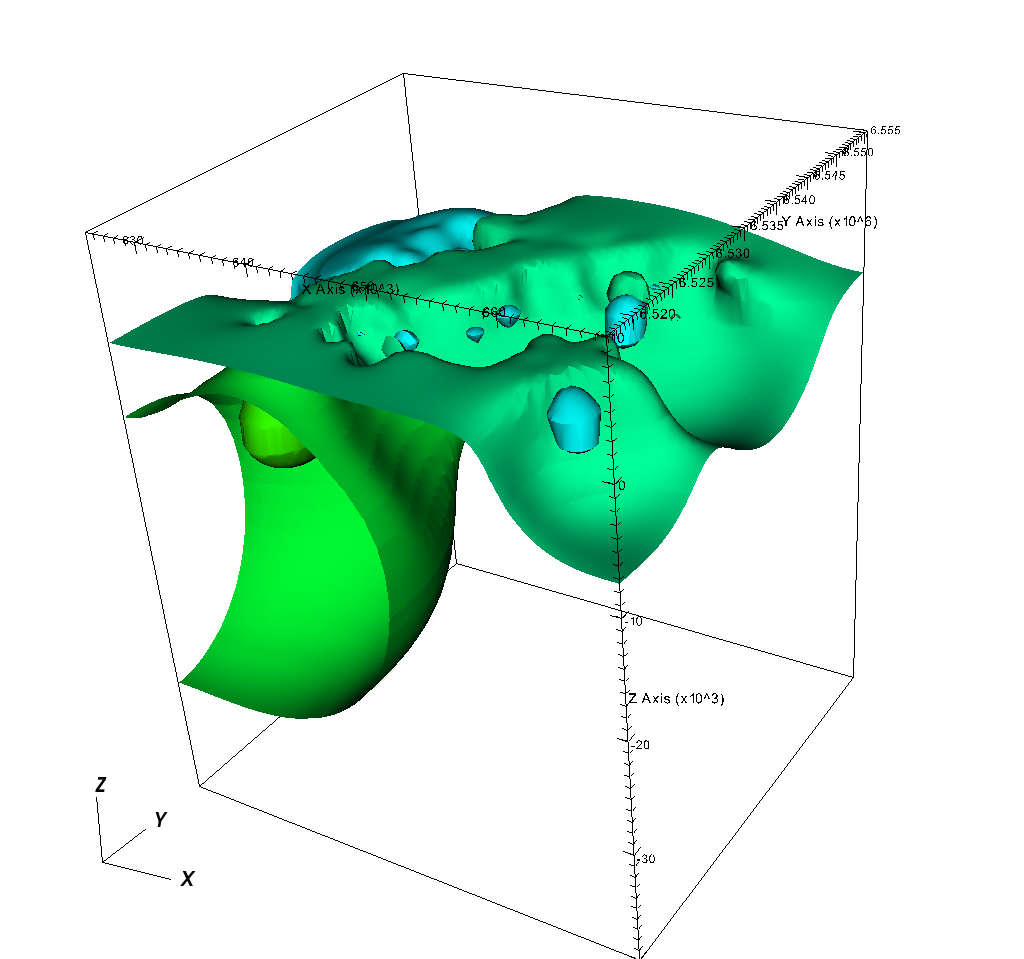
\includegraphics[width=\textwidth]{density1.png}
\caption{Contour image through a 3 dimensional gravity inversion which presents discrepancy in density. Its surrounded area is before the padding with uncertainty function. The gravity of padding area of the
model is not defined. Increasing and decreasing in density are indicated with red color and blue color respectively.}
\end{figure}

\begin{figure}
\centering
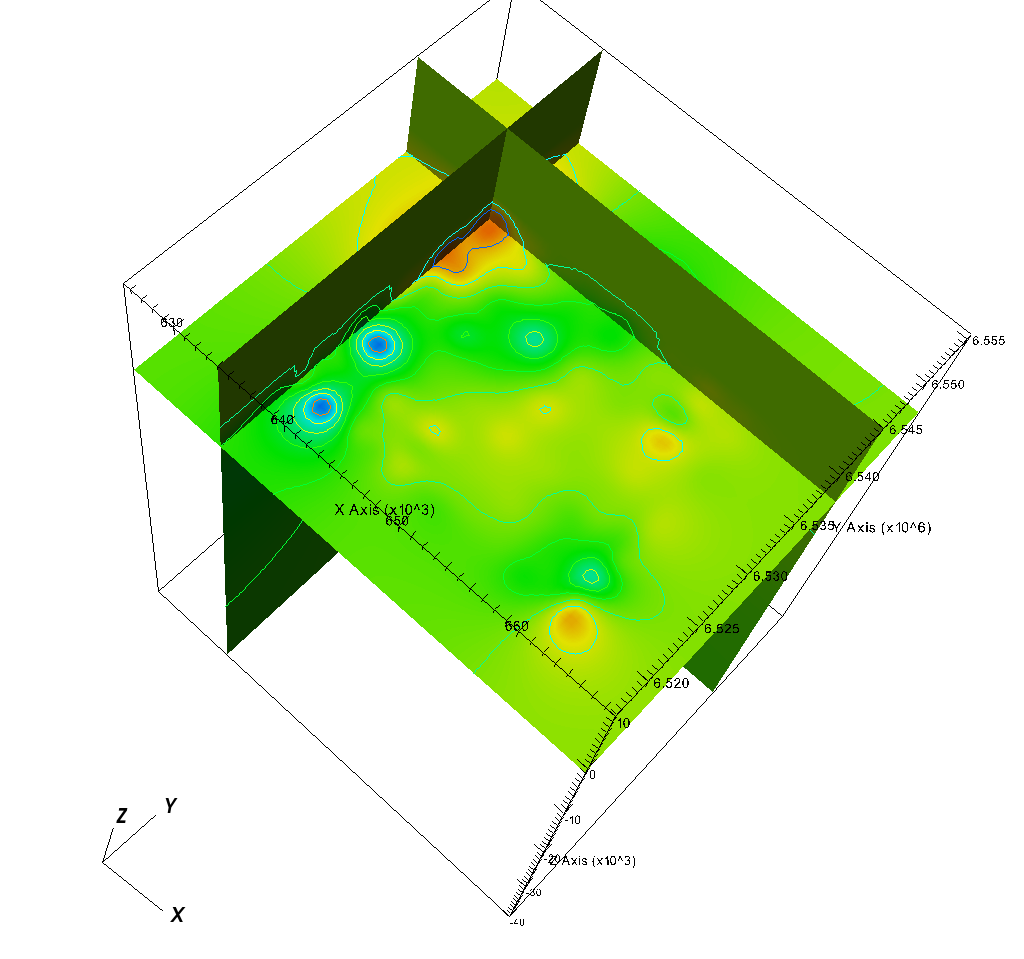
\includegraphics[width=\textwidth]{density2.png}
\caption{Depth image across previous 3D gravity inversion which presents discrepancy in density. Diversity in density are detected with colors and contours.}
\end{figure}

Such inversion calculations invariably depend on the characteristics of the forward modeling assumptions. From this point of view, it could be mentioned that traditional inversion is fundamentally based on a model of the subsurface which have used as a prior knowledge.

This inversion method is contained iterations inversion approach which use a series of improvement on a basic model in order to fit the result with the input data. Eventually the result after desirable iterations and error factor and providing satisfactory fitting to given data, is as a final model.


\section{Gravity Data}

Theoretically weighs depends on the force of gravity at that position and the force of gravity varies with elevation, rock densities, latitude and topography. Mass, however, does not depend on gravity but is a constitutive quantity throughout the earth. So the spring stretch in mass suspension is related to the gravity force. In addition with a constant mass, difference in spring stretch illustrate the changes in acceleration of gravity. The principal of gravity exploration is based on the topography of the basement, thickness of the sedimentary section with various density, porosity of the layer and elevation.

The amount of $g$ at sea level is about 980 $kg/s^2$ or 980,000 $mgal$. Gravity acceleration is measured in two types. The first corresponds to specify the absolute magnitude of gravity at any place and the second refers to the alteration in gravity from one place to another. In gravity study variation of this value which is caused by underground structure, is plotted as a residual gravity. Closed variation in residual gravity indicates discrepancy in subsurface geological structure.

The Gravity data are taken from onshore and offshore observation recorded at many gravity stations with high precision of determination in elevation and position (latitude and longitude). All Raw reading gravity observations require to process with many corrections.

The sun and moon gravitational forces make curvature in Earth's shape. These tide effects change figure of oceans, atmosphere and even solid body of the Earth, which impress gravity measurement and it is necessary to compensate it, which vary with location, date and time of the day.

The surface of the Earth is lumpy on land and water. However for Geophysical and Geological study, a smooth closed surface is assumed. The main one is a spheroid flattened at the poles which is called ellipsoid. The new data are used to defined a best-fitting obtained ellipsoid. The second suggestion is geoid which is really mathematical convenience. There is a uniform mass between gravity stations and ellipsoid, that's effect must be removed with corrections.

Also the level of topography for hilly and valley measurements is important. The gravity amount which is made up by that equal the mass of hill or valley must be added as a terrain correction to have a measurement on a level surface.

Because gravity descend towards the poles the latitude correction must be added to the observed gravity.

Free-air correction that must be added to observation, ignores the effects of material between the measurement and reference level which is positive for above sea-level station and is negative for station below sea-level.

The gravitational acceleration or Bouguer correction is calculated for known thickness (between measurements station and ellipsoid) and density (depends on local rock) which must be subtracted from the measurements gravity if station is above sea-level. and the station is below sea-level this must be added.

For this adjustment first of all Tidal correction apply based on tidal table or calculated tidal effect for given time and location of gravity data. The second one is terrain correction. Then Latitude, Free air and Bouguer correction have applied. The standard Bouguer density is 2670 $kg/m^3$.

(in the input file, bouguer anomaly is used as residual gravity  which have to be gridded.)



\section{Input File} 

For starting up the inversion 2 files are needed. Each of the two files contains a series of parameters which must appear in the correct order, as described in the next paragraph. Each parameter is marked by a keyword, which is followed either on the same line or the next line by one or more parameter values. 

The first file is contained the gravity anomaly, including number of points, the accurate location (latitude and longitude) of the observed position and the value of the anomaly after all gravity corrections. The main part in collecting the data is spacing of the observation point which means that all data must be gridded and its spacing affected the simulation resolution wisely.

The second is run_gravity with py extension which is related to the codes though it needs some constraints to have a good results in inversion.

A small part of sample of run_gravity:

\begin{verbatim}
mu=100
THICKNESS=20.*U.km
DATASET='QLD_west.nc'
PAD_X = 0.2
PAD_Y = 0.2
l_air = 6. * U.km
n_cells_v = 25
\end{verbatim}

Run_gravity file consist many options to implement which control how inversion is performed such as padding area, depth , MU factor,\ldots.

\begin{description} 	
\item[MAX\_ITER]
Specifying maximum iteration depends on model and the area which have been selected to have an inversion in it and your hard capacity. However the best result were built with 200 iterations. In addition all steps of inversion could be traced and the suited one selected.

\item[l_pad or PAD\_X, PAD\_Y] To implement the boundary constraints in this file, padding area in $x$ and $y$ direction should be determined. In a rectangular area, same padding for both direction is preferable. If directional area will be fixed with elongation in one orientation it does not matter to change the padding area. In addition for 2D inversion padding just add in one direction.

\item[DATASET] In run_gravity file just the location and the name of the data file have to be fixed. Both source of data and run_gravity files must be in a folder. 

\item[THICKNESS] Depth of the model should be assigned to have dipper or shallower inversion also it is assigned to the layer where shows inversion in.The parameter values must be real numbers, and they represent depths in km.

\item[l_air] Length of air is height of the model above the sea level. 

\item[n_cells_v] The last important part of the inversion property is the number of elements in data of the model which shows the finer or coarser cells in the model so its delimitation have affected on resolution of the inversion.

\item[mu]It is defined in accordance with the noise of data and it has a wide range to select from 0.0001 to 100 for each inversion.

\end{description}

\section{Output File}

At the end of each inversion iteration, package produces a new inversion file with 'gravin.silo' name which is stored in the file. This silo file shows the inversion result which does not have the number of iterations stage.

 In terminal indicates the specifications of inversion iterations. In this descriptions of the paths of all inversion during stages of modeling are cleared. The format of the file will be described here as it is designed to be used directly for analysis or debugging.

After final iteration the silo file, the result of inversion, is visible with some software which shows silo file format. It illuminate density distribution in the area (not in the padding) which create the gravity input data.

\section{Reference}

There are three examples for 2D and 3D gravity inversions with artificial input data.
In first step, an area with synthetic density section was suggested. Then based on forward modeling its gravitational data was collected. Afterwards with generated gravity data, escripts simulated a volume of inverted density. Whilst new density mass could be compared with the synthetic density section to verify the inversion.

Some of the presumptions were the same for all of the examples to simplify the situation to make a logical comparison between synthetic input and output. which is as followed:

\begin{verbatim}
n_cells_in_data=100
depth_offset=0.*U.km
l_data = 100 * U.km
l_pad=40*U.km
THICKNESS=20.*U.km
l_air=6*U.km
\end{verbatim}

The others assumptions comes with each examples.
\begin{enumerate}
\item  A 2D density section with a maximum in center was assumed. The reference density and inverted will be shown. The padding area is excluded. (\ref{fig:gravity2D1})

\begin{verbatim}
n_cells_in_data=100
n_humbs_h= 1
n_humbs_v=1
mu=100
\end{verbatim}

\begin{figure}
\centering
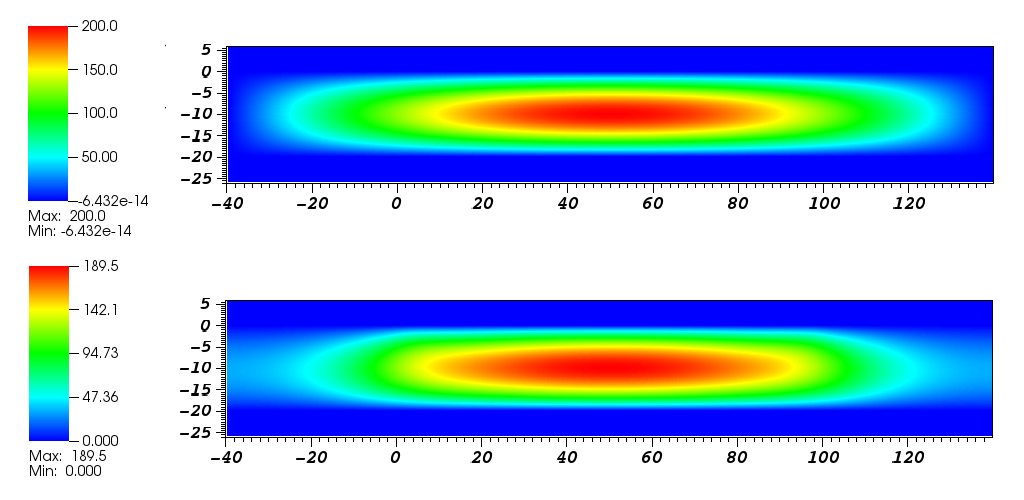
\includegraphics[width=\textwidth]{grav2D1.png}
\caption{2D density model up) reference    down) result}
\label{fig:gravity2D1}
\end{figure}


\item A 2D density properties with two maximum in corners and one minimum in the center was inverted. The result have eliminated the effects in padding area.(\ref{fig:gravity2D3}) 

\begin{verbatim}
n_cells_in_data=100
n_humbs_h= 3
n_humbs_v=1
mu=100
\end{verbatim}

\begin{figure}
\centering
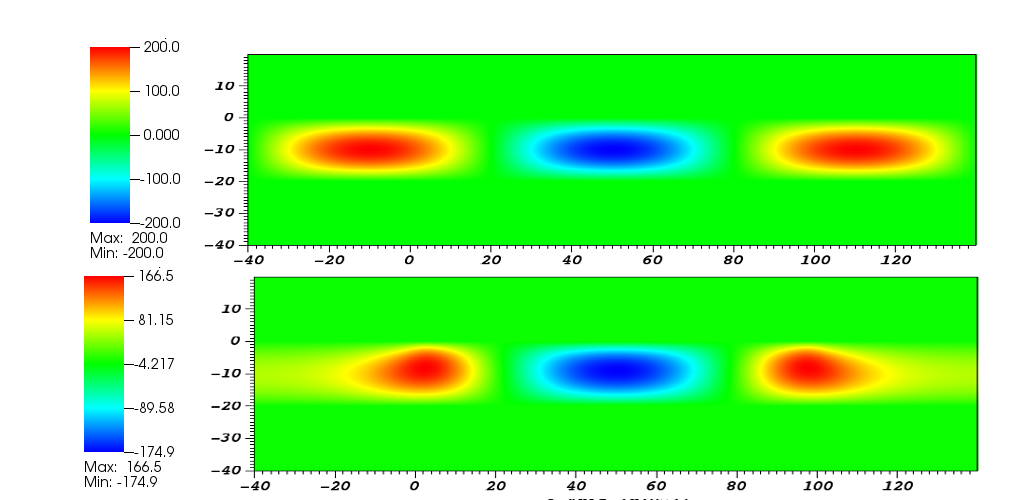
\includegraphics[width=\textwidth]{grav2D3.png}
\caption{2D density model up) reference  down) result}
\label{fig:gravity2D3}
\end{figure}

\item A 3D model with a maximum in the center was used as input data and the result after simulation in shown in the next image which determined a good distribution of density through the model in the main area.(\ref{fig:gravity3D} and \ref{fig:gravity3D1})

\begin{verbatim}
n_cells_in_data=50
n_humbs_h= 1
n_humbs_v=1
mu=10
\end{verbatim}

\begin{figure}
\centering
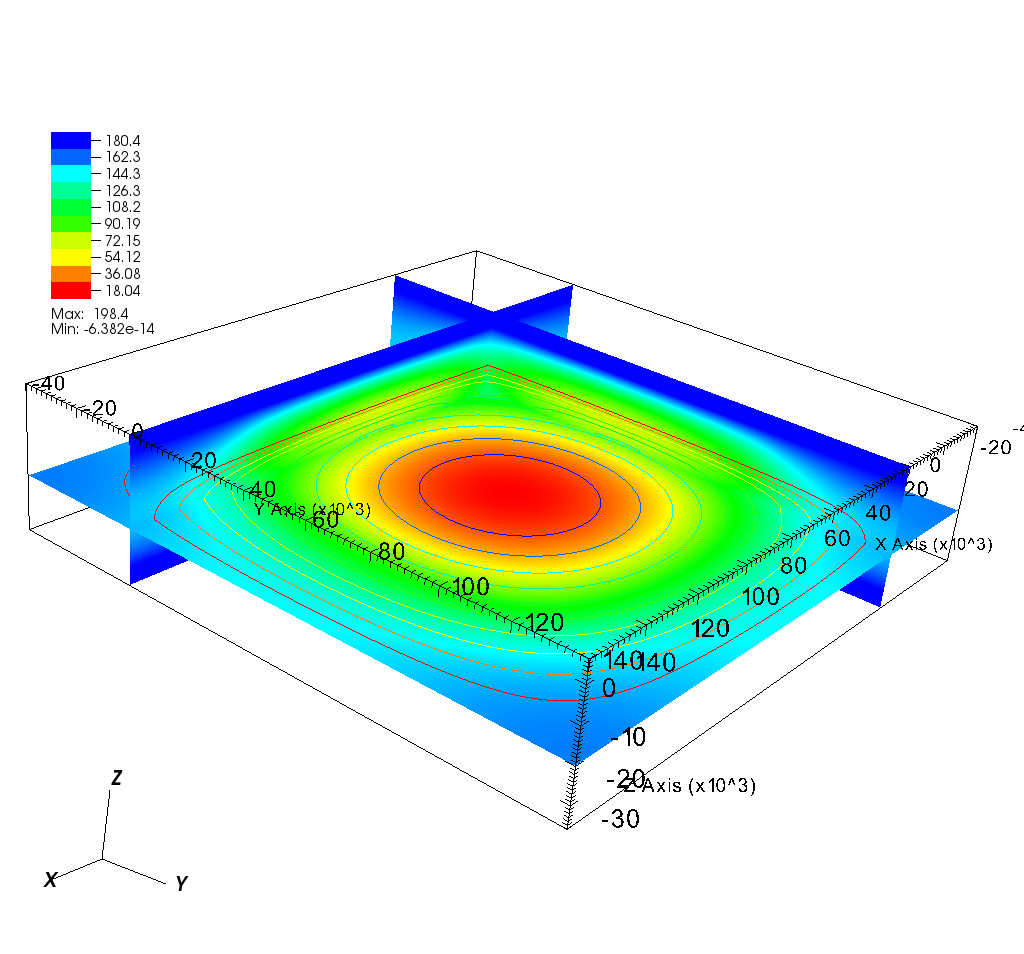
\includegraphics[width=\textwidth]{density3D-ref.png}
\caption{3D density model of reference as synthetic data}
\label{fig:gravity3D}
\end{figure}

\begin{figure}
\centering
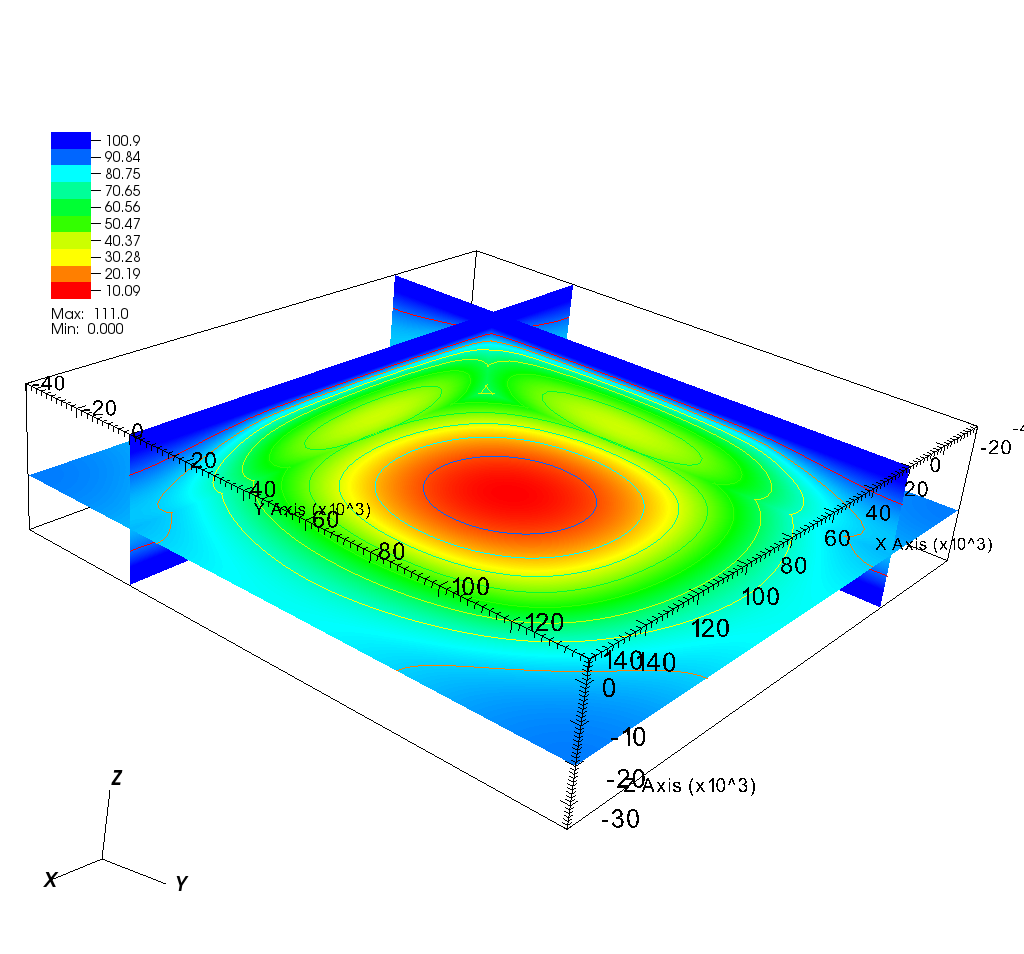
\includegraphics[width=\textwidth]{gravity3D.png}
\caption{3D density model of result}
\label{fig:gravity3D1}
\end{figure}
\end{enumerate}
